%!TeX root=../tese.tex
%("dica" para o editor de texto: este arquivo é parte de um documento maior)
% para saber mais: https://tex.stackexchange.com/q/78101/183146

%% ------------------------------------------------------------------------- %%
\chapter{Algoritmo Guloso}
\label{cap:algoritmo-guloso}

Neste capítulo entenderemos como a visão geométrica de um algoritmo de busca em ABB para uma sequência de acessos $X$ se relaciona com o custo ótimo OPT(X). Além disso, será apresentado um algoritmo guloso offline que transforma um conjunto arboreamente insatisfeito em um conjunto arboreamente satisfeito adicionando uma série de pontos, tentando adicionar o menor número possível de pontos ao conjunto. Por fim, argumentaremos como esse algoritmo pode ser adaptado para um algoritmo online em ABBs dentro do modelo de computação adotado.

\section{Otimalidade} 

Revisemos a definição de custo nesse modelo de computação. O custo para realizar um acesso é o número de nós visitados durante esse acesso. Assim, $OPT(X)$ é o menor custo necessário para um algoritmo de busca offline em ABB realizar todos os acessos de uma entrada $X = (x_{1},\ldots,x_{m})$, ou seja, o número mínimo de visitas a nós necessárias para realizar todos os acessos.

Retornando à análise geométrica, seja $P$ um conjunto de pontos. Denotaremos por \textit{minASS(P)} o tamanho do menor conjunto arboreamente satisfeito que contém $P$. 

Seja $P$ a visão geométrica do algoritmo de busca em ABB que possui custo $OPT(X)$ para a sequência de acessos $X$. De acordo com o Lema~\ref{lema:visao_geometrica_vira_ASS}, $P$ é um conjunto arboreamente satisfeito. Além disso, $|P|$ é mínimo para a entrada $X$, pois $P$ é a visão geométrica do algoritmo de busca em ABB que possui o custo ótimo $OPT(X)$. Assim, nota-se que $OPT(X) = minASS(V(X))$, sendo $V(X)$ a visão geométrica da entrada $X$.

Isso implica que o problema de encontrar o custo de um algoritmo ótimo de busca em ABBs para uma sequência de acessos $X$ pode ser reformulado como o problema de encontrar o menor superconjunto arboreamente satisfeito do conjunto $P_X$.

\section{Guloso futurista}

Apesar de não se saber se é possível encontrar o valor de $OPT(X)$ em tempo polinomial, e consequentemente encontrar o menor subconjunto de $P_X$ arboreamente satisfeito, apresentaremos o algoritmo Guloso futurista - Greedy Future - que dado o conjunto $P_X$ de pontos que representa a sequência $X$ de acessos, produz um conjunto pequeno de pontos $P$ que contém $P_X$ e que é arboreamente satisfeito. 

Naturalmente $|P_X| \geq |X| = m$ e todos os pontos de $P_X$ possuem coordenadas $y$ distintas dentro do intervalo $[1,m]$. 

O algoritmo funciona da seguinte maneira: inicialmente defina uma reta horizontal $r$ em $y = 1$ e inicialize $P = P_X$. Seja $a \in P \cap r$ um ponto com coordenadas $(a.x, a.y)$. Para cada $\{a,b\}$-retângulo insatisfeito em $P$, com $b$ um ponto com coordenadas $(b.x, b.y)$, com $b.y < a.y$, adicione um ponto em $(b.x, a.y)$. Após satisfazer todos os $\{a,b\}$-retângulos desse tipo, mova $r$ uma unidade para cima e repita. O algoritmo termina após satisfazer todos os $\{a,b\}$-retângulos com $r$ em $y = m$. Veja a Figura~\ref{fig:GreedyFuture-funcionamento}.

\begin{figure}
    \centering
    
    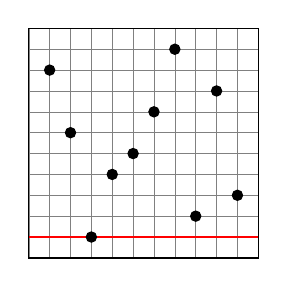
\begin{tikzpicture}[scale=0.265]
        \draw[very thin, gray] (0,0) grid (11,11);
        
        \draw[red, thick] (0,1) -- (11,1);

        \filldraw[black] (3,1) circle (7pt);
        \filldraw[black] (8,2) circle (7pt);
        \filldraw[black] (10,3) circle (7pt);
        \filldraw[black] (4,4) circle (7pt);
        \filldraw[black] (5,5) circle (7pt);
        \filldraw[black] (2,6) circle (7pt);
        \filldraw[black] (6,7) circle (7pt);
        \filldraw[black] (9,8) circle (7pt);
        \filldraw[black] (1,9) circle (7pt);
        \filldraw[black] (7,10) circle (7pt);
        \draw[black, line width=0.5pt] (0,0) rectangle (11,11);
    \end{tikzpicture}
    \hfill 
    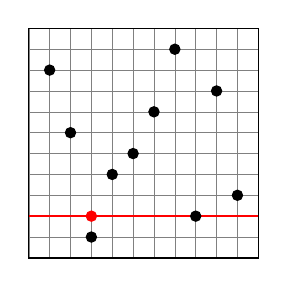
\begin{tikzpicture}[scale=0.265]
        \draw[very thin, gray] (0,0) grid (11,11);
        
        \draw[red, thick] (0,2) -- (11,2);

        \filldraw[black] (3,1) circle (7pt);
        \filldraw[black] (8,2) circle (7pt);
        \filldraw[black] (10,3) circle (7pt);
        \filldraw[black] (4,4) circle (7pt);
        \filldraw[black] (5,5) circle (7pt);
        \filldraw[black] (2,6) circle (7pt);
        \filldraw[black] (6,7) circle (7pt);
        \filldraw[black] (9,8) circle (7pt);
        \filldraw[black] (1,9) circle (7pt);
        \filldraw[black] (7,10) circle (7pt);
        \filldraw[red] (3,2) circle (7pt);

        \draw[black, line width=0.5pt] (0,0) rectangle (11,11);
    \end{tikzpicture}
    \hfill 
    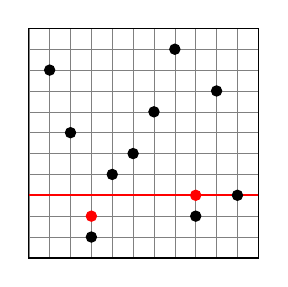
\begin{tikzpicture}[scale=0.265]
        \draw[very thin, gray] (0,0) grid (11,11);
        
        \draw[red, thick] (0,3) -- (11,3);

        \filldraw[black] (3,1) circle (7pt);
        \filldraw[black] (8,2) circle (7pt);
        \filldraw[black] (10,3) circle (7pt);
        \filldraw[black] (4,4) circle (7pt);
        \filldraw[black] (5,5) circle (7pt);
        \filldraw[black] (2,6) circle (7pt);
        \filldraw[black] (6,7) circle (7pt);
        \filldraw[black] (9,8) circle (7pt);
        \filldraw[black] (1,9) circle (7pt);
        \filldraw[black] (7,10) circle (7pt);
        \filldraw[red] (3,2) circle (7pt);
        \filldraw[red] (8,3) circle (7pt);
        \draw[black, line width=0.5pt] (0,0) rectangle (11,11);
    \end{tikzpicture}
    \hfill 
    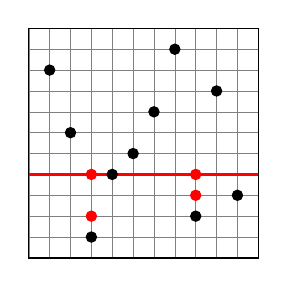
\begin{tikzpicture}[scale=0.265]
        \draw[very thin, gray] (0,0) grid (11,11);
        
        \draw[red, thick] (0,4) -- (11,4);

        \filldraw[black] (3,1) circle (7pt);
        \filldraw[black] (8,2) circle (7pt);
        \filldraw[black] (10,3) circle (7pt);
        \filldraw[black] (4,4) circle (7pt);
        \filldraw[black] (5,5) circle (7pt);
        \filldraw[black] (2,6) circle (7pt);
        \filldraw[black] (6,7) circle (7pt);
        \filldraw[black] (9,8) circle (7pt);
        \filldraw[black] (1,9) circle (7pt);
        \filldraw[black] (7,10) circle (7pt);
        \filldraw[red] (3,2) circle (7pt);
        \filldraw[red] (8,3) circle (7pt);
        \filldraw[red] (3,4) circle (7pt);
        \filldraw[red] (8,4) circle (7pt);
        \draw[black, line width=0.5pt] (0,0) rectangle (11,11); 
    \end{tikzpicture}
    \hfill 
    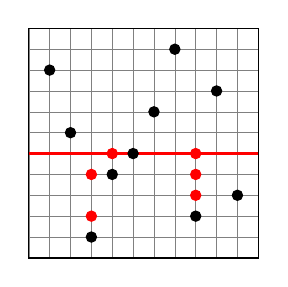
\begin{tikzpicture}[scale=0.265]
        \draw[very thin, gray] (0,0) grid (11,11);
        
        \draw[red, thick] (0,5) -- (11,5);

        \filldraw[black] (3,1) circle (7pt);
        \filldraw[black] (8,2) circle (7pt);
        \filldraw[black] (10,3) circle (7pt);
        \filldraw[black] (4,4) circle (7pt);
        \filldraw[black] (5,5) circle (7pt);
        \filldraw[black] (2,6) circle (7pt);
        \filldraw[black] (6,7) circle (7pt);
        \filldraw[black] (9,8) circle (7pt);
        \filldraw[black] (1,9) circle (7pt);
        \filldraw[black] (7,10) circle (7pt);
        \filldraw[red] (3,2) circle (7pt);
        \filldraw[red] (8,3) circle (7pt);
        \filldraw[red] (3,4) circle (7pt);
        \filldraw[red] (8,4) circle (7pt);
        \filldraw[red] (4,5) circle (7pt);
        \filldraw[red] (8,5) circle (7pt);
        \draw[black, line width=0.5pt] (0,0) rectangle (11,11); 
    \end{tikzpicture}
    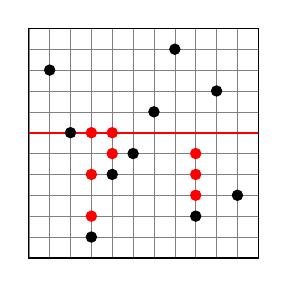
\begin{tikzpicture}[scale=0.265]
        \draw[very thin, gray] (0,0) grid (11,11);
        
        \draw[red, thick] (0,6) -- (11,6);

        \filldraw[black] (3,1) circle (7pt);
        \filldraw[black] (8,2) circle (7pt);
        \filldraw[black] (10,3) circle (7pt);
        \filldraw[black] (4,4) circle (7pt);
        \filldraw[black] (5,5) circle (7pt);
        \filldraw[black] (2,6) circle (7pt);
        \filldraw[black] (6,7) circle (7pt);
        \filldraw[black] (9,8) circle (7pt);
        \filldraw[black] (1,9) circle (7pt);
        \filldraw[black] (7,10) circle (7pt);
        \filldraw[red] (3,2) circle (7pt);
        \filldraw[red] (8,3) circle (7pt);
        \filldraw[red] (3,4) circle (7pt);
        \filldraw[red] (8,4) circle (7pt);
        \filldraw[red] (4,5) circle (7pt);
        \filldraw[red] (8,5) circle (7pt);
        \filldraw[red] (3,6) circle (7pt);
        \filldraw[red] (4,6) circle (7pt);
        \draw[black, line width=0.5pt] (0,0) rectangle (11,11); 
    \end{tikzpicture}
    \hfill 
    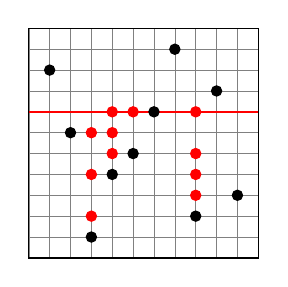
\begin{tikzpicture}[scale=0.265]
        \draw[very thin, gray] (0,0) grid (11,11);
        
        \draw[red, thick] (0,7) -- (11,7);

        \filldraw[black] (3,1) circle (7pt);
        \filldraw[black] (8,2) circle (7pt);
        \filldraw[black] (10,3) circle (7pt);
        \filldraw[black] (4,4) circle (7pt);
        \filldraw[black] (5,5) circle (7pt);
        \filldraw[black] (2,6) circle (7pt);
        \filldraw[black] (6,7) circle (7pt);
        \filldraw[black] (9,8) circle (7pt);
        \filldraw[black] (1,9) circle (7pt);
        \filldraw[black] (7,10) circle (7pt);
        \filldraw[red] (3,2) circle (7pt);
        \filldraw[red] (8,3) circle (7pt);
        \filldraw[red] (3,4) circle (7pt);
        \filldraw[red] (8,4) circle (7pt);
        \filldraw[red] (4,5) circle (7pt);
        \filldraw[red] (8,5) circle (7pt);
        \filldraw[red] (3,6) circle (7pt);
        \filldraw[red] (4,6) circle (7pt);
        \filldraw[red] (4,7) circle (7pt);
        \filldraw[red] (5,7) circle (7pt);
        \filldraw[red] (8,7) circle (7pt);
        \draw[black, line width=0.5pt] (0,0) rectangle (11,11); 
    \end{tikzpicture}
    \hfill 
    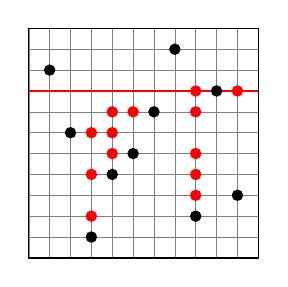
\begin{tikzpicture}[scale=0.265]
        \draw[very thin, gray] (0,0) grid (11,11);
        
        \draw[red, thick] (0,8) -- (11,8);

        \filldraw[black] (3,1) circle (7pt);
        \filldraw[black] (8,2) circle (7pt);
        \filldraw[black] (10,3) circle (7pt);
        \filldraw[black] (4,4) circle (7pt);
        \filldraw[black] (5,5) circle (7pt);
        \filldraw[black] (2,6) circle (7pt);
        \filldraw[black] (6,7) circle (7pt);
        \filldraw[black] (9,8) circle (7pt);
        \filldraw[black] (1,9) circle (7pt);
        \filldraw[black] (7,10) circle (7pt);
        \filldraw[red] (3,2) circle (7pt);
        \filldraw[red] (8,3) circle (7pt);
        \filldraw[red] (3,4) circle (7pt);
        \filldraw[red] (8,4) circle (7pt);
        \filldraw[red] (4,5) circle (7pt);
        \filldraw[red] (8,5) circle (7pt);
        \filldraw[red] (3,6) circle (7pt);
        \filldraw[red] (4,6) circle (7pt);
        \filldraw[red] (4,7) circle (7pt);
        \filldraw[red] (5,7) circle (7pt);
        \filldraw[red] (8,7) circle (7pt);
        \filldraw[red] (8,8) circle (7pt);
        \filldraw[red] (10,8) circle (7pt);
        \draw[black, line width=0.5pt] (0,0) rectangle (11,11); 
    \end{tikzpicture}
    \hfill 
    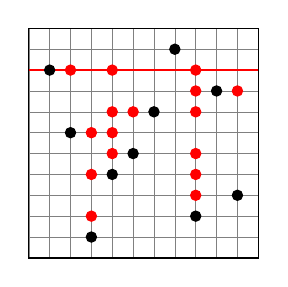
\begin{tikzpicture}[scale=0.265]
        \draw[very thin, gray] (0,0) grid (11,11);
        
        \draw[red, thick] (0,9) -- (11,9);

        \filldraw[black] (3,1) circle (7pt);
        \filldraw[black] (8,2) circle (7pt);
        \filldraw[black] (10,3) circle (7pt);
        \filldraw[black] (4,4) circle (7pt);
        \filldraw[black] (5,5) circle (7pt);
        \filldraw[black] (2,6) circle (7pt);
        \filldraw[black] (6,7) circle (7pt);
        \filldraw[black] (9,8) circle (7pt);
        \filldraw[black] (1,9) circle (7pt);
        \filldraw[black] (7,10) circle (7pt);
        \filldraw[red] (3,2) circle (7pt);
        \filldraw[red] (8,3) circle (7pt);
        \filldraw[red] (3,4) circle (7pt);
        \filldraw[red] (8,4) circle (7pt);
        \filldraw[red] (4,5) circle (7pt);
        \filldraw[red] (8,5) circle (7pt);
        \filldraw[red] (3,6) circle (7pt);
        \filldraw[red] (4,6) circle (7pt);
        \filldraw[red] (4,7) circle (7pt);
        \filldraw[red] (5,7) circle (7pt);
        \filldraw[red] (8,7) circle (7pt);
        \filldraw[red] (8,8) circle (7pt);
        \filldraw[red] (10,8) circle (7pt);
        \filldraw[red] (2,9) circle (7pt);
        \filldraw[red] (4,9) circle (7pt);
        \filldraw[red] (8,9) circle (7pt);
        \draw[black, line width=0.5pt] (0,0) rectangle (11,11); 
    \end{tikzpicture}
    \hfill 
    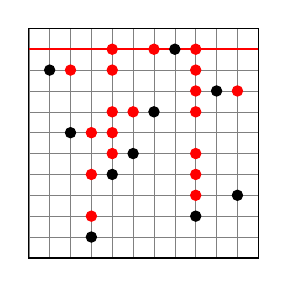
\begin{tikzpicture}[scale=0.265]
        % Desenha o quadriculado
        \draw[very thin, gray] (0,0) grid (11,11);
        
        \draw[red, thick] (0,10) -- (11,10);

        \filldraw[black] (3,1) circle (7pt);
        \filldraw[black] (8,2) circle (7pt);
        \filldraw[black] (10,3) circle (7pt);
        \filldraw[black] (4,4) circle (7pt);
        \filldraw[black] (5,5) circle (7pt);
        \filldraw[black] (2,6) circle (7pt);
        \filldraw[black] (6,7) circle (7pt);
        \filldraw[black] (9,8) circle (7pt);
        \filldraw[black] (1,9) circle (7pt);
        \filldraw[black] (7,10) circle (7pt);
        \filldraw[red] (3,2) circle (7pt);
        \filldraw[red] (8,3) circle (7pt);
        \filldraw[red] (3,4) circle (7pt);
        \filldraw[red] (8,4) circle (7pt);
        \filldraw[red] (4,5) circle (7pt);
        \filldraw[red] (8,5) circle (7pt);
        \filldraw[red] (3,6) circle (7pt);
        \filldraw[red] (4,6) circle (7pt);
        \filldraw[red] (4,7) circle (7pt);
        \filldraw[red] (5,7) circle (7pt);
        \filldraw[red] (8,7) circle (7pt);
        \filldraw[red] (8,8) circle (7pt);
        \filldraw[red] (10,8) circle (7pt);
        \filldraw[red] (2,9) circle (7pt);
        \filldraw[red] (4,9) circle (7pt);
        \filldraw[red] (8,9) circle (7pt);
        \filldraw[red] (4,10) circle (7pt);
        \filldraw[red] (8,10) circle (7pt);
        \filldraw[red] (6,10) circle (7pt);
        \draw[black, line width=0.5pt] (0,0) rectangle (11,11); 
    \end{tikzpicture}
    \caption{Execução do Greedy Future para a sequência X = (3,8,10,4,5,2,6,9,1,7) de acessos.}
\label{fig:GreedyFuture-funcionamento}
\end{figure}

O algoritmo mantém o invariante que ao final da iteração do algoritmo para a reta horizontal $y = l$, todos os pares de ponto $\{a,b\}$, com $a,b \in P$ e $a.y, b.y \leq l$ são arboreamente satisfeitos. Assim, por construção, o resultado do algoritmo é um conjunto aboreamente satisfeito.

%De maneira prática, o algoritmo analisa os pontos de $P$ na reta horizontal $r$ com $y = i$, com $i \in \{1,\ldots,m\}$ de maneira crescente. Assim, após satisfazer todos os pontos com coordenada $y = i$, sabemos que todos os pares de pontos que estão abaixo ou na reta $r$ estão satisfeitos. Assim, por construção, o resultado do algoritmo é um conjunto arboreamente satisfeito.

O comportamento desse algoritmo é caracterizado por uma abordagem gulosa local. Veremos que esse algoritmo quando refletido no contexto de ABBs visita apenas as chaves que estão no caminho da chave buscada e reorganiza todos os nós visitados de maneira a deixar mais perto da raiz, as próximas chaves a serem visitados, e consequentemente, mais longe da raiz as chaves a serem visitados mais tarde. 

Embora o algoritmo garanta encontrar uma solução válida, ou seja, um conjunto $P$ arboreamente satisfeito, o Guloso futurista não garante que $|P| = minASS$. Veja a Figura~\ref{fig:greedy_subotimo}.

\begin{figure}
    \centering
    
    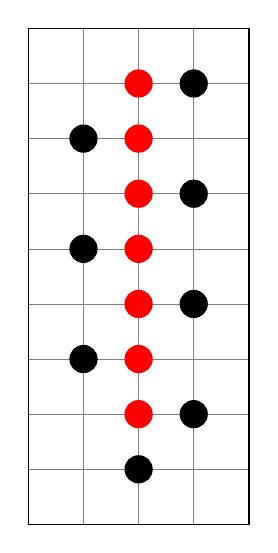
\begin{tikzpicture}[scale=0.7]
        \draw[very thin, gray] (0,0) grid (4,9);

        \filldraw[black] (2,1) circle (7pt);
        \filldraw[black] (3,2) circle (7pt);
        \filldraw[black] (1,3) circle (7pt);
        \filldraw[black] (3,4) circle (7pt);
        \filldraw[black] (1,5) circle (7pt);
        \filldraw[black] (3,6) circle (7pt);
        \filldraw[black] (1,7) circle (7pt);
        \filldraw[black] (3,8) circle (7pt);
        \filldraw[red] (2,2) circle (7pt);
        \filldraw[red] (2,3) circle (7pt);
        \filldraw[red] (2,4) circle (7pt);
        \filldraw[red] (2,5) circle (7pt);
        \filldraw[red] (2,6) circle (7pt);
        \filldraw[red] (2,7) circle (7pt);
        \filldraw[red] (2,8) circle (7pt);
        
        \draw[black, line width=0.5pt] (0,0) rectangle (4,9);
    \end{tikzpicture}
    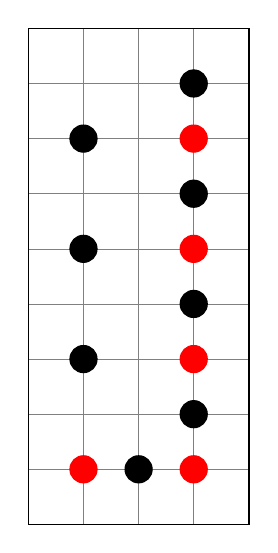
\begin{tikzpicture}[scale=0.7]
        \draw[very thin, gray] (0,0) grid (4,9);
        
        \filldraw[black] (2,1) circle (7pt);
        \filldraw[black] (3,2) circle (7pt);
        \filldraw[black] (1,3) circle (7pt);
        \filldraw[black] (3,4) circle (7pt);
        \filldraw[black] (1,5) circle (7pt);
        \filldraw[black] (3,6) circle (7pt);
        \filldraw[black] (1,7) circle (7pt);
        \filldraw[black] (3,8) circle (7pt);
        \filldraw[red] (1,1) circle (7pt);
        \filldraw[red] (3,1) circle (7pt);
        \filldraw[red] (3,3) circle (7pt);
        \filldraw[red] (3,5) circle (7pt);
        \filldraw[red] (3,7) circle (7pt);
        
        \draw[black, line width=0.5pt] (0,0) rectangle (4,9);
    \end{tikzpicture}
    \caption{Em preto, os pontos de $P_X$ para uma sequência $X$ de acessos. À esquerda, o conjunto de pontos produzidos pelo Guloso futurista. À direita, o menor conjunto arboreamente satisfeito para $P_X$, de tamanho minASS($P_X$).}
\label{fig:greedy_subotimo}
\end{figure}

\begin{figure}
    \centering
    \begin{minipage}[b]{0.48\linewidth}
        \centering
        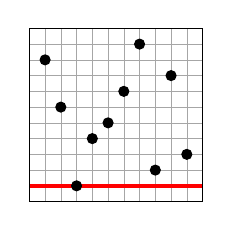
\begin{tikzpicture}[scale=0.2] %1
            \draw[very thin, gray!70] (0,0) grid (11,11);
            
            \draw[red, line width=1.2pt] (0,1) -- (11,1);
    
            \filldraw[black] (3,1) circle (9pt);
            \filldraw[black] (8,2) circle (9pt);
            \filldraw[black] (10,3) circle (9pt);
            \filldraw[black] (4,4) circle (9pt);
            \filldraw[black] (5,5) circle (9pt);
            \filldraw[black] (2,6) circle (9pt);
            \filldraw[black] (6,7) circle (9pt);
            \filldraw[black] (9,8) circle (9pt);
            \filldraw[black] (1,9) circle (9pt);
            \filldraw[black] (7,10) circle (9pt);
            \draw[black, line width=0.5pt] (0,0) rectangle (11,11);
        \end{tikzpicture}
        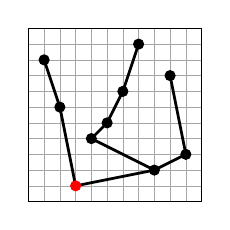
\begin{tikzpicture}[scale=0.2]
            \draw[very thin, gray!70] (0,0) grid (11,11);
            
            \draw[black, line width=1pt] (3,1) -- (8,2) -- (10,3) -- (9,8);
            \draw[black, line width=1pt] (3,1) -- (2,6) -- (1,9);
            \draw[black, line width=1pt] (8,2) -- (4,4) -- (5,5) -- (6,7) -- (7,10);
    
            \filldraw[red] (3,1) circle (9pt);
            \filldraw[black] (8,2) circle (9pt);
            \filldraw[black] (10,3) circle (9pt);
            \filldraw[black] (4,4) circle (9pt);
            \filldraw[black] (5,5) circle (9pt);
            \filldraw[black] (2,6) circle (9pt);
            \filldraw[black] (6,7) circle (9pt);
            \filldraw[black] (9,8) circle (9pt);
            \filldraw[black] (1,9) circle (9pt);
            \filldraw[black] (7,10) circle (9pt);
            \draw[black, line width=0.5pt] (0,0) rectangle (11,11);
        \end{tikzpicture}
        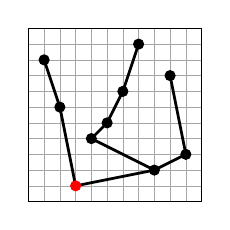
\begin{tikzpicture}[scale=0.2]
            \draw[very thin, gray!70] (0,0) grid (11,11);
            
            \draw[black, line width=1pt] (3,1) -- (8,2) -- (10,3) -- (9,8);
            \draw[black, line width=1pt] (3,1) -- (2,6) -- (1,9);
            \draw[black, line width=1pt] (8,2) -- (4,4) -- (5,5) -- (6,7) -- (7,10);
    
            \filldraw[red] (3,1) circle (9pt);
            \filldraw[black] (8,2) circle (9pt);
            \filldraw[black] (10,3) circle (9pt);
            \filldraw[black] (4,4) circle (9pt);
            \filldraw[black] (5,5) circle (9pt);
            \filldraw[black] (2,6) circle (9pt);
            \filldraw[black] (6,7) circle (9pt);
            \filldraw[black] (9,8) circle (9pt);
            \filldraw[black] (1,9) circle (9pt);
            \filldraw[black] (7,10) circle (9pt);
            \draw[black, line width=0.5pt] (0,0) rectangle (11,11);
        \end{tikzpicture}
        \\
        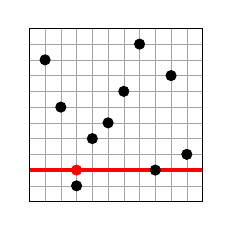
\begin{tikzpicture}[scale=0.2] %2
            \draw[very thin, gray!70] (0,0) grid (11,11);
            
            \draw[red, line width=1.2pt] (0,2) -- (11,2);
            
    
            \filldraw[black] (3,1) circle (9pt);
            \filldraw[black] (8,2) circle (9pt);
            \filldraw[black] (10,3) circle (9pt);
            \filldraw[black] (4,4) circle (9pt);
            \filldraw[black] (5,5) circle (9pt);
            \filldraw[black] (2,6) circle (9pt);
            \filldraw[black] (6,7) circle (9pt);
            \filldraw[black] (9,8) circle (9pt);
            \filldraw[black] (1,9) circle (9pt);
            \filldraw[black] (7,10) circle (9pt);
            \filldraw[red] (3,2) circle (9pt);
    
            \draw[black, line width=0.5pt] (0,0) rectangle (11,11);
        \end{tikzpicture}
        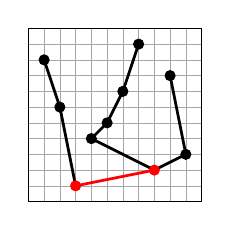
\begin{tikzpicture}[scale=0.2]
            \draw[very thin, gray!70] (0,0) grid (11,11);
            
            \draw[red, line width=1pt] (3,1) -- (8,2);
            \draw[black, line width=1pt] (8,2) -- (10,3);
            \draw[black, line width=1pt] (10,3) -- (9,8);
            \draw[black, line width=1pt] (3,1) -- (2,6) -- (1,9);
            \draw[black, line width=1pt] (8,2) -- (4,4) -- (5,5) -- (6,7) -- (7,10);
    
            \filldraw[red] (3,1) circle (9pt);
            \filldraw[red] (8,2) circle (9pt);
            \filldraw[black] (10,3) circle (9pt);
            \filldraw[black] (4,4) circle (9pt);
            \filldraw[black] (5,5) circle (9pt);
            \filldraw[black] (2,6) circle (9pt);
            \filldraw[black] (6,7) circle (9pt);
            \filldraw[black] (9,8) circle (9pt);
            \filldraw[black] (1,9) circle (9pt);
            \filldraw[black] (7,10) circle (9pt);
            \draw[black, line width=0.5pt] (0,0) rectangle (11,11);
        \end{tikzpicture}
        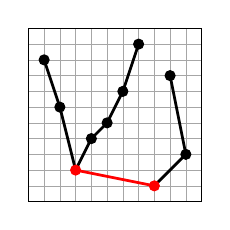
\begin{tikzpicture}[scale=0.2]
            \draw[very thin, gray!70] (0,0) grid (11,11);

            \draw[red, line width=1pt] (3,2) -- (8,1);
            \draw[black, line width=1pt] (8,1) -- (10,3) -- (9,8);
            \draw[black, line width=1pt] (3,2) -- (2,6) -- (1,9);
            \draw[black, line width=1pt] (3,2) -- (4,4) -- (5,5) -- (6,7) -- (7,10);
            
            \filldraw[red] (8,1) circle (9pt);
            \filldraw[red] (3,2) circle (9pt);
            \filldraw[black] (10,3) circle (9pt);
            \filldraw[black] (4,4) circle (9pt);
            \filldraw[black] (5,5) circle (9pt);
            \filldraw[black] (2,6) circle (9pt);
            \filldraw[black] (6,7) circle (9pt);
            \filldraw[black] (9,8) circle (9pt);
            \filldraw[black] (1,9) circle (9pt);
            \filldraw[black] (7,10) circle (9pt);
            \draw[black, line width=0.5pt] (0,0) rectangle (11,11);
        \end{tikzpicture}
        \\
        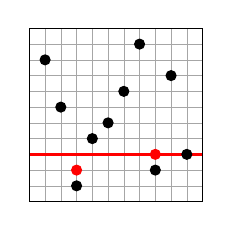
\begin{tikzpicture}[scale=0.2] %3
            \draw[very thin, gray!70] (0,0) grid (11,11);
            
            \draw[red, line width=1.2pt] (0,3) -- (11,3);
    
            \filldraw[black] (3,1) circle (9pt);
            \filldraw[black] (8,2) circle (9pt);
            \filldraw[black] (10,3) circle (9pt);
            \filldraw[black] (4,4) circle (9pt);
            \filldraw[black] (5,5) circle (9pt);
            \filldraw[black] (2,6) circle (9pt);
            \filldraw[black] (6,7) circle (9pt);
            \filldraw[black] (9,8) circle (9pt);
            \filldraw[black] (1,9) circle (9pt);
            \filldraw[black] (7,10) circle (9pt);
            \filldraw[red] (3,2) circle (9pt);
            \filldraw[red] (8,3) circle (9pt);
            \draw[black, line width=0.5pt] (0,0) rectangle (11,11);
        \end{tikzpicture}
        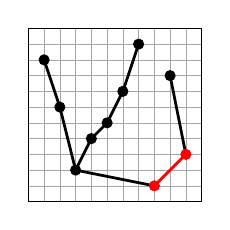
\begin{tikzpicture}[scale=0.2]
            \draw[very thin, gray!70] (0,0) grid (11,11);

            \draw[red, line width=1pt] (8,1) -- (10,3);
            \draw[black, line width=1pt] (10,3) -- (9,8);
            \draw[black, line width=1pt] (3,2) -- (2,6) -- (1,9);
            \draw[black, line width=1pt] (8,1) -- (3,2) -- (4,4) -- (5,5) -- (6,7) -- (7,10);

            \filldraw[red] (8,1) circle (9pt);
            \filldraw[black] (3,2) circle (9pt);
            \filldraw[red] (10,3) circle (9pt);
            \filldraw[black] (4,4) circle (9pt);
            \filldraw[black] (5,5) circle (9pt);
            \filldraw[black] (2,6) circle (9pt);
            \filldraw[black] (6,7) circle (9pt);
            \filldraw[black] (9,8) circle (9pt);
            \filldraw[black] (1,9) circle (9pt);
            \filldraw[black] (7,10) circle (9pt);
            \draw[black, line width=0.5pt] (0,0) rectangle (11,11);
        \end{tikzpicture}
        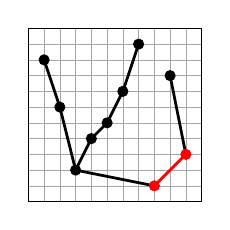
\begin{tikzpicture}[scale=0.2]
            \draw[very thin, gray!70] (0,0) grid (11,11);

            \draw[red, line width=1pt] (8,1) -- (10,3);
            \draw[black, line width=1pt] (10,3) -- (9,8);
            \draw[black, line width=1pt] (3,2) -- (2,6) -- (1,9);
            \draw[black, line width=1pt] (8,1) -- (3,2) -- (4,4) -- (5,5) -- (6,7) -- (7,10);

            \filldraw[red] (8,1) circle (9pt);
            \filldraw[black] (3,2) circle (9pt);
            \filldraw[red] (10,3) circle (9pt);
            \filldraw[black] (4,4) circle (9pt);
            \filldraw[black] (5,5) circle (9pt);
            \filldraw[black] (2,6) circle (9pt);
            \filldraw[black] (6,7) circle (9pt);
            \filldraw[black] (9,8) circle (9pt);
            \filldraw[black] (1,9) circle (9pt);
            \filldraw[black] (7,10) circle (9pt);
            \draw[black, line width=0.5pt] (0,0) rectangle (11,11);
        \end{tikzpicture}
        \\
        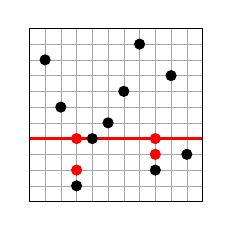
\begin{tikzpicture}[scale=0.2] %4
            \draw[very thin, gray!70] (0,0) grid (11,11);
            
            \draw[red, line width=1.2pt] (0,4) -- (11,4);
    
            \filldraw[black] (3,1) circle (9pt);
            \filldraw[black] (8,2) circle (9pt);
            \filldraw[black] (10,3) circle (9pt);
            \filldraw[black] (4,4) circle (9pt);
            \filldraw[black] (5,5) circle (9pt);
            \filldraw[black] (2,6) circle (9pt);
            \filldraw[black] (6,7) circle (9pt);
            \filldraw[black] (9,8) circle (9pt);
            \filldraw[black] (1,9) circle (9pt);
            \filldraw[black] (7,10) circle (9pt);
            \filldraw[red] (3,2) circle (9pt);
            \filldraw[red] (8,3) circle (9pt);
            \filldraw[red] (3,4) circle (9pt);
            \filldraw[red] (8,4) circle (9pt);
            \draw[black, line width=0.5pt] (0,0) rectangle (11,11); 
        \end{tikzpicture}
        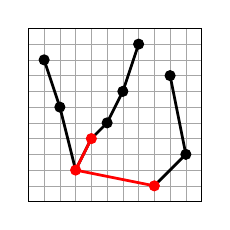
\begin{tikzpicture}[scale=0.2]
            \draw[very thin, gray!70] (0,0) grid (11,11);

            \draw[black, line width=1pt] (8,1) -- (10,3) -- (9,8);
            \draw[black, line width=1pt] (3,2) -- (2,6) -- (1,9);
            \draw[black, line width=1pt] (3,2) -- (4,4) -- (5,5) -- (6,7) -- (7,10);
            \draw[red, line width=1pt] (8,1) -- (3,2) -- (4,4);

            \filldraw[red] (8,1) circle (9pt);
            \filldraw[red] (3,2) circle (9pt);
            \filldraw[black] (10,3) circle (9pt);
            \filldraw[red] (4,4) circle (9pt);
            \filldraw[black] (5,5) circle (9pt);
            \filldraw[black] (2,6) circle (9pt);
            \filldraw[black] (6,7) circle (9pt);
            \filldraw[black] (9,8) circle (9pt);
            \filldraw[black] (1,9) circle (9pt);
            \filldraw[black] (7,10) circle (9pt);
            \draw[black, line width=0.5pt] (0,0) rectangle (11,11);
        \end{tikzpicture}
        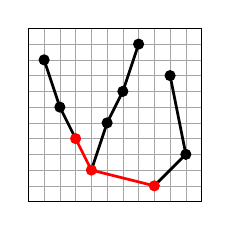
\begin{tikzpicture}[scale=0.2]
            \draw[very thin, gray!70] (0,0) grid (11,11);

            \draw[black, line width=1pt] (8,1) -- (10,3) -- (9,8);
            \draw[black, line width=1pt] (3,4) -- (2,6) -- (1,9);
            \draw[black, line width=1pt] (4,2) -- (5,5) -- (6,7) -- (7,10);
            \draw[red, line width=1pt] (8,1) -- (4,2) -- (3,4);

            \filldraw[red] (8,1) circle (9pt);
            \filldraw[red] (4,2) circle (9pt);
            \filldraw[black] (10,3) circle (9pt);
            \filldraw[red] (3,4) circle (9pt);
            \filldraw[black] (5,5) circle (9pt);
            \filldraw[black] (2,6) circle (9pt);
            \filldraw[black] (6,7) circle (9pt);
            \filldraw[black] (9,8) circle (9pt);
            \filldraw[black] (1,9) circle (9pt);
            \filldraw[black] (7,10) circle (9pt);
            \draw[black, line width=0.5pt] (0,0) rectangle (11,11);
        \end{tikzpicture}
        \\
        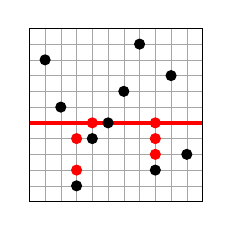
\begin{tikzpicture}[scale=0.2] %5
            \draw[very thin, gray!70] (0,0) grid (11,11);
            
            \draw[red, line width=1.2pt] (0,5) -- (11,5);
    
            \filldraw[black] (3,1) circle (9pt);
            \filldraw[black] (8,2) circle (9pt);
            \filldraw[black] (10,3) circle (9pt);
            \filldraw[black] (4,4) circle (9pt);
            \filldraw[black] (5,5) circle (9pt);
            \filldraw[black] (2,6) circle (9pt);
            \filldraw[black] (6,7) circle (9pt);
            \filldraw[black] (9,8) circle (9pt);
            \filldraw[black] (1,9) circle (9pt);
            \filldraw[black] (7,10) circle (9pt);
            \filldraw[red] (3,2) circle (9pt);
            \filldraw[red] (8,3) circle (9pt);
            \filldraw[red] (3,4) circle (9pt);
            \filldraw[red] (8,4) circle (9pt);
            \filldraw[red] (4,5) circle (9pt);
            \filldraw[red] (8,5) circle (9pt);
            \draw[black, line width=0.5pt] (0,0) rectangle (11,11); 
        \end{tikzpicture}
        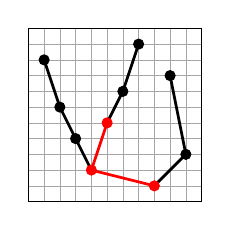
\begin{tikzpicture}[scale=0.2]
            \draw[very thin, gray!70] (0,0) grid (11,11);

            \draw[black, line width=1pt] (8,1) -- (10,3) -- (9,8);
            \draw[black, line width=1pt] (4,2) -- (3,4) -- (2,6) -- (1,9);
            \draw[black, line width=1pt] (5,5) -- (6,7) -- (7,10);
            \draw[red, line width=1pt] (8,1) -- (4,2) -- (5,5);

            \filldraw[red] (8,1) circle (9pt);
            \filldraw[red] (4,2) circle (9pt);
            \filldraw[black] (10,3) circle (9pt);
            \filldraw[black] (3,4) circle (9pt);
            \filldraw[red] (5,5) circle (9pt);
            \filldraw[black] (2,6) circle (9pt);
            \filldraw[black] (6,7) circle (9pt);
            \filldraw[black] (9,8) circle (9pt);
            \filldraw[black] (1,9) circle (9pt);
            \filldraw[black] (7,10) circle (9pt);
            \draw[black, line width=0.5pt] (0,0) rectangle (11,11);
        \end{tikzpicture}
        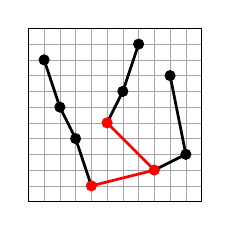
\begin{tikzpicture}[scale=0.2]
            \draw[very thin, gray!70] (0,0) grid (11,11);

            \draw[black, line width=1pt] (8,2) -- (10,3) -- (9,8);
            \draw[black, line width=1pt] (4,1) -- (3,4) -- (2,6) -- (1,9);
            \draw[black, line width=1pt] (5,5) -- (6,7) -- (7,10);
            \draw[red, line width=1pt] (4,1) -- (8,2) -- (5,5);

            \filldraw[red] (4,1) circle (9pt);
            \filldraw[red] (8,2) circle (9pt);
            \filldraw[black] (10,3) circle (9pt);
            \filldraw[black] (3,4) circle (9pt);
            \filldraw[red] (5,5) circle (9pt);
            \filldraw[black] (2,6) circle (9pt);
            \filldraw[black] (6,7) circle (9pt);
            \filldraw[black] (9,8) circle (9pt);
            \filldraw[black] (1,9) circle (9pt);
            \filldraw[black] (7,10) circle (9pt);
            \draw[black, line width=0.5pt] (0,0) rectangle (11,11);
        \end{tikzpicture}
    \end{minipage}
    %\hspace{0.01\linewidth}
    \hfill
    \begin{minipage}[b]{0.48\linewidth}
        \centering
        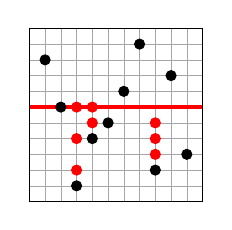
\begin{tikzpicture}[scale=0.2] %6
            \draw[very thin, gray!70] (0,0) grid (11,11);
            
            \draw[red, line width=1.2pt] (0,6) -- (11,6);
    
            \filldraw[black] (3,1) circle (9pt);
            \filldraw[black] (8,2) circle (9pt);
            \filldraw[black] (10,3) circle (9pt);
            \filldraw[black] (4,4) circle (9pt);
            \filldraw[black] (5,5) circle (9pt);
            \filldraw[black] (2,6) circle (9pt);
            \filldraw[black] (6,7) circle (9pt);
            \filldraw[black] (9,8) circle (9pt);
            \filldraw[black] (1,9) circle (9pt);
            \filldraw[black] (7,10) circle (9pt);
            \filldraw[red] (3,2) circle (9pt);
            \filldraw[red] (8,3) circle (9pt);
            \filldraw[red] (3,4) circle (9pt);
            \filldraw[red] (8,4) circle (9pt);
            \filldraw[red] (4,5) circle (9pt);
            \filldraw[red] (8,5) circle (9pt);
            \filldraw[red] (3,6) circle (9pt);
            \filldraw[red] (4,6) circle (9pt);
            \draw[black, line width=0.5pt] (0,0) rectangle (11,11); 
        \end{tikzpicture}
        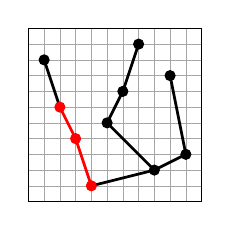
\begin{tikzpicture}[scale=0.2]
            \draw[very thin, gray!70] (0,0) grid (11,11);

            \draw[black, line width=1pt] (8,2) -- (10,3) -- (9,8);
            \draw[red, line width=1pt] (4,1) -- (3,4) -- (2,6);
            \draw[black, line width=1pt] (2,6) -- (1,9);
            \draw[black, line width=1pt] (5,5) -- (6,7) -- (7,10);
            \draw[black, line width=1pt] (4,1) -- (8,2) -- (5,5);

            \filldraw[red] (4,1) circle (9pt);
            \filldraw[black] (8,2) circle (9pt);
            \filldraw[black] (10,3) circle (9pt);
            \filldraw[red] (3,4) circle (9pt);
            \filldraw[black] (5,5) circle (9pt);
            \filldraw[red] (2,6) circle (9pt);
            \filldraw[black] (6,7) circle (9pt);
            \filldraw[black] (9,8) circle (9pt);
            \filldraw[black] (1,9) circle (9pt);
            \filldraw[black] (7,10) circle (9pt);
            \draw[black, line width=0.5pt] (0,0) rectangle (11,11);
        \end{tikzpicture}
        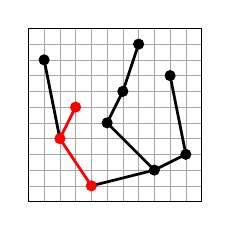
\begin{tikzpicture}[scale=0.2]
            \draw[very thin, gray!70] (0,0) grid (11,11);

            \draw[black, line width=1pt] (8,2) -- (10,3) -- (9,8);
            \draw[red, line width=1pt] (4,1) -- (2,4) -- (3,6);
            \draw[black, line width=1pt] (2,4) -- (1,9);
            \draw[black, line width=1pt] (5,5) -- (6,7) -- (7,10);
            \draw[black, line width=1pt] (4,1) -- (8,2) -- (5,5);

            \filldraw[red] (4,1) circle (9pt);
            \filldraw[black] (8,2) circle (9pt);
            \filldraw[black] (10,3) circle (9pt);
            \filldraw[red] (2,4) circle (9pt);
            \filldraw[black] (5,5) circle (9pt);
            \filldraw[red] (3,6) circle (9pt);
            \filldraw[black] (6,7) circle (9pt);
            \filldraw[black] (9,8) circle (9pt);
            \filldraw[black] (1,9) circle (9pt);
            \filldraw[black] (7,10) circle (9pt);
            \draw[black, line width=0.5pt] (0,0) rectangle (11,11);
        \end{tikzpicture}
        \\
        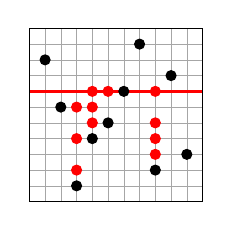
\begin{tikzpicture}[scale=0.2] %7
            \draw[very thin, gray!70] (0,0) grid (11,11);
            
            \draw[red, line width=1.2pt] (0,7) -- (11,7);
    
            \filldraw[black] (3,1) circle (9pt);
            \filldraw[black] (8,2) circle (9pt);
            \filldraw[black] (10,3) circle (9pt);
            \filldraw[black] (4,4) circle (9pt);
            \filldraw[black] (5,5) circle (9pt);
            \filldraw[black] (2,6) circle (9pt);
            \filldraw[black] (6,7) circle (9pt);
            \filldraw[black] (9,8) circle (9pt);
            \filldraw[black] (1,9) circle (9pt);
            \filldraw[black] (7,10) circle (9pt);
            \filldraw[red] (3,2) circle (9pt);
            \filldraw[red] (8,3) circle (9pt);
            \filldraw[red] (3,4) circle (9pt);
            \filldraw[red] (8,4) circle (9pt);
            \filldraw[red] (4,5) circle (9pt);
            \filldraw[red] (8,5) circle (9pt);
            \filldraw[red] (3,6) circle (9pt);
            \filldraw[red] (4,6) circle (9pt);
            \filldraw[red] (4,7) circle (9pt);
            \filldraw[red] (5,7) circle (9pt);
            \filldraw[red] (8,7) circle (9pt);
            \draw[black, line width=0.5pt] (0,0) rectangle (11,11); 
        \end{tikzpicture}
        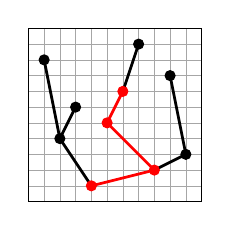
\begin{tikzpicture}[scale=0.2]
            \draw[very thin, gray!70] (0,0) grid (11,11);

            \draw[black, line width=1pt] (8,2) -- (10,3) -- (9,8);
            \draw[black, line width=1pt] (4,1) -- (2,4) -- (3,6);
            \draw[black, line width=1pt] (2,4) -- (1,9);
            \draw[black, line width=1pt] (6,7) -- (7,10);
            \draw[red, line width=1pt] (4,1) -- (8,2) -- (5,5) -- (6,7);

            \filldraw[red] (4,1) circle (9pt);
            \filldraw[red] (8,2) circle (9pt);
            \filldraw[black] (10,3) circle (9pt);
            \filldraw[black] (2,4) circle (9pt);
            \filldraw[red] (5,5) circle (9pt);
            \filldraw[black] (3,6) circle (9pt);
            \filldraw[red] (6,7) circle (9pt);
            \filldraw[black] (9,8) circle (9pt);
            \filldraw[black] (1,9) circle (9pt);
            \filldraw[black] (7,10) circle (9pt);
            \draw[black, line width=0.5pt] (0,0) rectangle (11,11);
        \end{tikzpicture}
        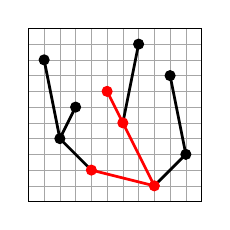
\begin{tikzpicture}[scale=0.2]
            \draw[very thin, gray!70] (0,0) grid (11,11);

            \draw[black, line width=1pt] (8,1) -- (10,3) -- (9,8);
            \draw[black, line width=1pt] (4,2) -- (2,4) -- (3,6);
            \draw[black, line width=1pt] (2,4) -- (1,9);
            \draw[black, line width=1pt] (6,5) -- (7,10);
            \draw[red, line width=1pt] (4,2) -- (8,1) -- (6,5) -- (5,7);

            \filldraw[red] (8,1) circle (9pt);
            \filldraw[red] (4,2) circle (9pt);
            \filldraw[black] (10,3) circle (9pt);
            \filldraw[black] (2,4) circle (9pt);
            \filldraw[red] (6,5) circle (9pt);
            \filldraw[black] (3,6) circle (9pt);
            \filldraw[red] (5,7) circle (9pt);
            \filldraw[black] (9,8) circle (9pt);
            \filldraw[black] (1,9) circle (9pt);
            \filldraw[black] (7,10) circle (9pt);
            \draw[black, line width=0.5pt] (0,0) rectangle (11,11);
        \end{tikzpicture}       
        \\
        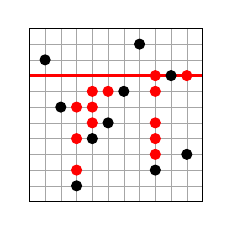
\begin{tikzpicture}[scale=0.2] %8
            \draw[very thin, gray!70] (0,0) grid (11,11);
            
            \draw[red, line width=1.2pt] (0,8) -- (11,8);
    
            \filldraw[black] (3,1) circle (9pt);
            \filldraw[black] (8,2) circle (9pt);
            \filldraw[black] (10,3) circle (9pt);
            \filldraw[black] (4,4) circle (9pt);
            \filldraw[black] (5,5) circle (9pt);
            \filldraw[black] (2,6) circle (9pt);
            \filldraw[black] (6,7) circle (9pt);
            \filldraw[black] (9,8) circle (9pt);
            \filldraw[black] (1,9) circle (9pt);
            \filldraw[black] (7,10) circle (9pt);
            \filldraw[red] (3,2) circle (9pt);
            \filldraw[red] (8,3) circle (9pt);
            \filldraw[red] (3,4) circle (9pt);
            \filldraw[red] (8,4) circle (9pt);
            \filldraw[red] (4,5) circle (9pt);
            \filldraw[red] (8,5) circle (9pt);
            \filldraw[red] (3,6) circle (9pt);
            \filldraw[red] (4,6) circle (9pt);
            \filldraw[red] (4,7) circle (9pt);
            \filldraw[red] (5,7) circle (9pt);
            \filldraw[red] (8,7) circle (9pt);
            \filldraw[red] (8,8) circle (9pt);
            \filldraw[red] (10,8) circle (9pt);
            \draw[black, line width=0.5pt] (0,0) rectangle (11,11); 
        \end{tikzpicture}
        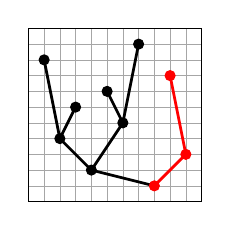
\begin{tikzpicture}[scale=0.2]
            \draw[very thin, gray!70] (0,0) grid (11,11);

            \draw[black, line width=1pt] (8,1) -- (4,2) -- (2,4) -- (3,6);
            \draw[black, line width=1pt] (2,4) -- (1,9);
            \draw[black, line width=1pt] (4,2) -- (6,5) -- (7,10);
            \draw[black, line width=1pt] (6,5) -- (5,7);
            \draw[red, line width=1pt] (8,1) -- (10,3) -- (9,8);

            \filldraw[red] (8,1) circle (9pt);
            \filldraw[black] (4,2) circle (9pt);
            \filldraw[red] (10,3) circle (9pt);
            \filldraw[black] (2,4) circle (9pt);
            \filldraw[black] (6,5) circle (9pt);
            \filldraw[black] (3,6) circle (9pt);
            \filldraw[black] (5,7) circle (9pt);
            \filldraw[red] (9,8) circle (9pt);
            \filldraw[black] (1,9) circle (9pt);
            \filldraw[black] (7,10) circle (9pt);
            \draw[black, line width=0.5pt] (0,0) rectangle (11,11);
        \end{tikzpicture}  
        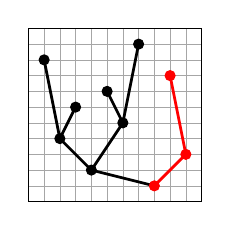
\begin{tikzpicture}[scale=0.2]
            \draw[very thin, gray!70] (0,0) grid (11,11);

            \draw[black, line width=1pt] (8,1) -- (4,2) -- (2,4) -- (3,6);
            \draw[black, line width=1pt] (2,4) -- (1,9);
            \draw[black, line width=1pt] (4,2) -- (6,5) -- (7,10);
            \draw[black, line width=1pt] (6,5) -- (5,7);
            \draw[red, line width=1pt] (8,1) -- (10,3) -- (9,8);

            \filldraw[red] (8,1) circle (9pt);
            \filldraw[black] (4,2) circle (9pt);
            \filldraw[red] (10,3) circle (9pt);
            \filldraw[black] (2,4) circle (9pt);
            \filldraw[black] (6,5) circle (9pt);
            \filldraw[black] (3,6) circle (9pt);
            \filldraw[black] (5,7) circle (9pt);
            \filldraw[red] (9,8) circle (9pt);
            \filldraw[black] (1,9) circle (9pt);
            \filldraw[black] (7,10) circle (9pt);
            \draw[black, line width=0.5pt] (0,0) rectangle (11,11);
        \end{tikzpicture}
        \\
        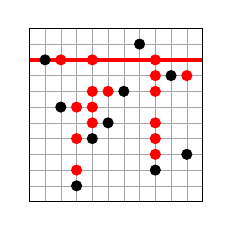
\begin{tikzpicture}[scale=0.2] %9
            \draw[very thin, gray!70] (0,0) grid (11,11);
            
            \draw[red, line width=1.2pt] (0,9) -- (11,9);
    
            \filldraw[black] (3,1) circle (9pt);
            \filldraw[black] (8,2) circle (9pt);
            \filldraw[black] (10,3) circle (9pt);
            \filldraw[black] (4,4) circle (9pt);
            \filldraw[black] (5,5) circle (9pt);
            \filldraw[black] (2,6) circle (9pt);
            \filldraw[black] (6,7) circle (9pt);
            \filldraw[black] (9,8) circle (9pt);
            \filldraw[black] (1,9) circle (9pt);
            \filldraw[black] (7,10) circle (9pt);
            \filldraw[red] (3,2) circle (9pt);
            \filldraw[red] (8,3) circle (9pt);
            \filldraw[red] (3,4) circle (9pt);
            \filldraw[red] (8,4) circle (9pt);
            \filldraw[red] (4,5) circle (9pt);
            \filldraw[red] (8,5) circle (9pt);
            \filldraw[red] (3,6) circle (9pt);
            \filldraw[red] (4,6) circle (9pt);
            \filldraw[red] (4,7) circle (9pt);
            \filldraw[red] (5,7) circle (9pt);
            \filldraw[red] (8,7) circle (9pt);
            \filldraw[red] (8,8) circle (9pt);
            \filldraw[red] (10,8) circle (9pt);
            \filldraw[red] (2,9) circle (9pt);
            \filldraw[red] (4,9) circle (9pt);
            \filldraw[red] (8,9) circle (9pt);
            \draw[black, line width=0.5pt] (0,0) rectangle (11,11); 
        \end{tikzpicture}
        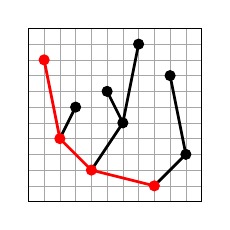
\begin{tikzpicture}[scale=0.2]
            \draw[very thin, gray!70] (0,0) grid (11,11);

            \draw[black, line width=1pt] (2,4) -- (3,6);
            \draw[red, line width=1pt] (8,1) -- (4,2) -- (2,4) -- (1,9);
            \draw[black, line width=1pt] (4,2) -- (6,5) -- (7,10);
            \draw[black, line width=1pt] (6,5) -- (5,7);
            \draw[black, line width=1pt] (8,1) -- (10,3) -- (9,8);

            \filldraw[red] (8,1) circle (9pt);
            \filldraw[red] (4,2) circle (9pt);
            \filldraw[black] (10,3) circle (9pt);
            \filldraw[red] (2,4) circle (9pt);
            \filldraw[black] (6,5) circle (9pt);
            \filldraw[black] (3,6) circle (9pt);
            \filldraw[black] (5,7) circle (9pt);
            \filldraw[black] (9,8) circle (9pt);
            \filldraw[red] (1,9) circle (9pt);
            \filldraw[black] (7,10) circle (9pt);
            \draw[black, line width=0.5pt] (0,0) rectangle (11,11);
        \end{tikzpicture}
        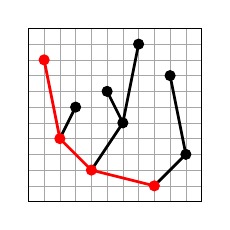
\begin{tikzpicture}[scale=0.2]
            \draw[very thin, gray!70] (0,0) grid (11,11);

            \draw[black, line width=1pt] (2,4) -- (3,6);
            \draw[red, line width=1pt] (8,1) -- (4,2) -- (2,4) -- (1,9);
            \draw[black, line width=1pt] (4,2) -- (6,5) -- (7,10);
            \draw[black, line width=1pt] (6,5) -- (5,7);
            \draw[black, line width=1pt] (8,1) -- (10,3) -- (9,8);

            \filldraw[red] (8,1) circle (9pt);
            \filldraw[red] (4,2) circle (9pt);
            \filldraw[black] (10,3) circle (9pt);
            \filldraw[red] (2,4) circle (9pt);
            \filldraw[black] (6,5) circle (9pt);
            \filldraw[black] (3,6) circle (9pt);
            \filldraw[black] (5,7) circle (9pt);
            \filldraw[black] (9,8) circle (9pt);
            \filldraw[red] (1,9) circle (9pt);
            \filldraw[black] (7,10) circle (9pt);
            \draw[black, line width=0.5pt] (0,0) rectangle (11,11);
        \end{tikzpicture}
        \\
        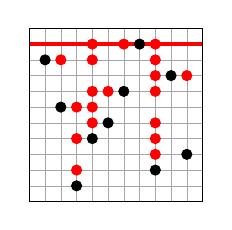
\begin{tikzpicture}[scale=0.2] %10
            \draw[very thin, gray!70] (0,0) grid (11,11);
            
            \draw[red, line width=1.2pt] (0,10) -- (11,10);
    
            \filldraw[black] (3,1) circle (9pt);
            \filldraw[black] (8,2) circle (9pt);
            \filldraw[black] (10,3) circle (9pt);
            \filldraw[black] (4,4) circle (9pt);
            \filldraw[black] (5,5) circle (9pt);
            \filldraw[black] (2,6) circle (9pt);
            \filldraw[black] (6,7) circle (9pt);
            \filldraw[black] (9,8) circle (9pt);
            \filldraw[black] (1,9) circle (9pt);
            \filldraw[black] (7,10) circle (9pt);
            \filldraw[red] (3,2) circle (9pt);
            \filldraw[red] (8,3) circle (9pt);
            \filldraw[red] (3,4) circle (9pt);
            \filldraw[red] (8,4) circle (9pt);
            \filldraw[red] (4,5) circle (9pt);
            \filldraw[red] (8,5) circle (9pt);
            \filldraw[red] (3,6) circle (9pt);
            \filldraw[red] (4,6) circle (9pt);
            \filldraw[red] (4,7) circle (9pt);
            \filldraw[red] (5,7) circle (9pt);
            \filldraw[red] (8,7) circle (9pt);
            \filldraw[red] (8,8) circle (9pt);
            \filldraw[red] (10,8) circle (9pt);
            \filldraw[red] (2,9) circle (9pt);
            \filldraw[red] (4,9) circle (9pt);
            \filldraw[red] (8,9) circle (9pt);
            \filldraw[red] (4,10) circle (9pt);
            \filldraw[red] (8,10) circle (9pt);
            \filldraw[red] (6,10) circle (9pt);
            \draw[black, line width=0.5pt] (0,0) rectangle (11,11); 
        \end{tikzpicture}
        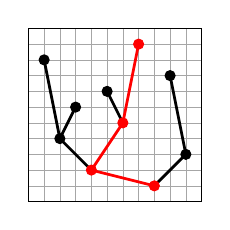
\begin{tikzpicture}[scale=0.2]
            \draw[very thin, gray!70] (0,0) grid (11,11);

            \draw[black, line width=1pt] (2,4) -- (3,6);
            \draw[red, line width=1pt] (8,1) -- (4,2) -- (6,5) -- (7,10);
            \draw[black, line width=1pt] (4,2) -- (2,4) -- (1,9);
            \draw[black, line width=1pt] (6,5) -- (5,7);
            \draw[black, line width=1pt] (8,1) -- (10,3) -- (9,8);

            \filldraw[red] (8,1) circle (9pt);
            \filldraw[red] (4,2) circle (9pt);
            \filldraw[black] (10,3) circle (9pt);
            \filldraw[black] (2,4) circle (9pt);
            \filldraw[red] (6,5) circle (9pt);
            \filldraw[black] (3,6) circle (9pt);
            \filldraw[black] (5,7) circle (9pt);
            \filldraw[black] (9,8) circle (9pt);
            \filldraw[black] (1,9) circle (9pt);
            \filldraw[red] (7,10) circle (9pt);
            \draw[black, line width=0.5pt] (0,0) rectangle (11,11);
        \end{tikzpicture}
        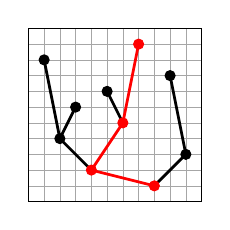
\begin{tikzpicture}[scale=0.2]
            \draw[very thin, gray!70] (0,0) grid (11,11);

            \draw[black, line width=1pt] (2,4) -- (3,6);
            \draw[red, line width=1pt] (8,1) -- (4,2) -- (6,5) -- (7,10);
            \draw[black, line width=1pt] (4,2) -- (2,4) -- (1,9);
            \draw[black, line width=1pt] (6,5) -- (5,7);
            \draw[black, line width=1pt] (8,1) -- (10,3) -- (9,8);

            \filldraw[red] (8,1) circle (9pt);
            \filldraw[red] (4,2) circle (9pt);
            \filldraw[black] (10,3) circle (9pt);
            \filldraw[black] (2,4) circle (9pt);
            \filldraw[red] (6,5) circle (9pt);
            \filldraw[black] (3,6) circle (9pt);
            \filldraw[black] (5,7) circle (9pt);
            \filldraw[black] (9,8) circle (9pt);
            \filldraw[black] (1,9) circle (9pt);
            \filldraw[red] (7,10) circle (9pt);
            \draw[black, line width=0.5pt] (0,0) rectangle (11,11);
        \end{tikzpicture}
    \end{minipage}
    \caption{Imagem nova.}
\label{fig:greedy_em_ ABB}
\end{figure}